\documentclass[tikz,border=8pt]{standalone}
\usepackage{amsmath}
\usepackage{pgfplots}
\pgfplotsset{compat=1.18}
\begin{document}
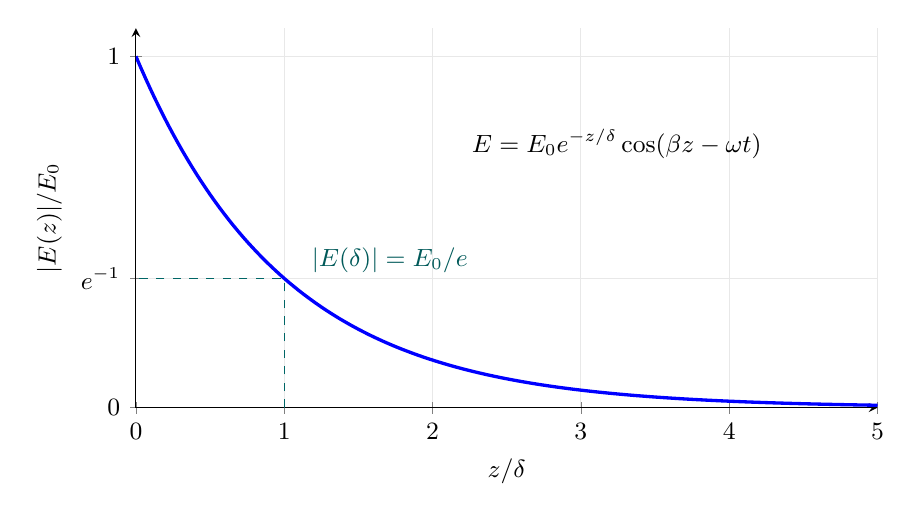
\begin{tikzpicture}[font=\sffamily\small]
\begin{axis}[
  width=11cm,height=6.4cm,
  axis lines=left,xmin=0,xmax=5,ymin=0,ymax=1.08,
  xlabel={$z/\delta$},ylabel={$|E(z)|/E_0$},
  xtick={0,1,2,3,4,5},ytick={0,0.367879,1},
  yticklabels={$0$,$e^{-1}$,$1$},
  grid=both,grid style={gray!18},
  every axis plot/.append style={very thick}]
  \addplot[blue,domain=0:5,samples=160]{exp(-x)};
  \draw[dashed,teal!80!black] (axis cs:1,0)--(axis cs:1,0.367879)
    --(axis cs:0,0.367879);
  \node[anchor=west,teal!70!black] at (axis cs:1.12,.42)
    {$|E(\delta)|=E_0/e$};
  \node[anchor=west] at (axis cs:2.2,.75)
    {$E=E_0e^{-z/\delta}\cos(\beta z-\omega t)$};
\end{axis}
\end{tikzpicture}
\end{document}
